\documentclass[journal,onecolumn]{IEEEtran}
% \usepackage[subpreambles=true]{standalone}
\usepackage{import}
\usepackage{blindtext}
% The preceding line is only needed to identify funding in the first footnote. If that is unneeded, please comment it out.
\usepackage{cite}
\usepackage{amsmath,amssymb,amsfonts,}
\usepackage{algorithmic}
\usepackage{graphicx}
\usepackage{textcomp}
\usepackage{dsfont}
\usepackage{bbm}
\usepackage{xcolor}
\usepackage{Mycustommath}
\usepackage{mathalpha}
\usepackage{relsize}
\usepackage{graphicx}
\usepackage[center]{caption}
\usepackage{hyperref}
\usepackage{color} 
\usepackage{fancyvrb} 


\begin{document}
\title{Toolbox harmonique : V0.1}
\maketitle
\today 

\section{Notations et convention}

\subsection{Représentation harmonique, phaseurs et évaluation temporelle d'une matrice temps périodique}

Soit $T \, \in \, \R^{*+}$, $ M(t) \in \C^{n_1 \times n_2}$ $T$-périodique

On définit la \emph{short time fourier transform} de $M(\cdot)$ par la séquence :
\begin{equation}
\F M  = (\hm M_{k})_{k\in \Z} \, ; \,\hm  M_{k} \in \C^{m,n}
\end{equation}
où $\hm M_{k}$ est donné par la formule : 
\begin{equation}
\hm M_{k} = \frac{1}{T} \int_{0}^{T} M(\tau) e^{-j k \frac{2\pi}{T} \tau }\mathrm{d}\tau 
\end{equation}

On note $\left((\hm M |_{m})_{k}\right)_{k\in [-m,m]}$ la troncature à l'ordre $m$ de la séquence $(\hm M_{k})$. 


On représente alors par un tableau à trois entrée (formellement un tenseur) $\hm M|_{m}$ : $\mathfrak{M}$, dont la troisieme dimension stocke les phaseurs de $M|m$.

\begin{equation}
\begin{cases}
\mathfrak{M}(i,j,m+1+k) = \frac{1}{T} \int_{0}^{T} M_{i,j}(\tau) e^{-j k \frac{2\pi}{T} \tau }\mathrm{d}\tau \\ 
(i,j) \in [1:n_1] \times[ 1:n_2], k \in [-m:m]
\end{cases}
\end{equation}

Ainsi sous \textsc{Matlab}, on utilisera les 3D-array pour le stockage des phaseurs d'une matrice périodique. 

L'évaluation temporelle de la matrice $M(t)$ se calcule alors grace au produit contracté mode-3 

\begin{equation}
\begin{cases}
(e_{i}(t))_{i\in [1 : 2m+1]} \in \C^{2m+1} \Leftrightarrow e_{m+1+k}(t) = e^{j k \frac{2 \pi }{T}}t \\
M(t) = \mathfrak{M} \cpmoden3 e =\sum_{l =1}^{2m+1} \mathfrak{M}(:,:,l) e_l(t)
\end{cases}
\end{equation}


sous \textsc{Matlab} la fonction \href{ https://fr.mathworks.com/help/matlab/ref/tensorprod.html }{\texttt{tensorprod}, disponible depuis la 2022ra} permet d'exprimer le produit de 2 tenseur et à fortiori le produit contracté en précisant les dimensions à faire coincider. 
% This file was automatically created from the m-file 
% "m2tex.m" written by USL. 
% The fontencoding in this file is UTF-8. 
%  
% You will need to include the following two packages in 
% your LaTeX-Main-File. 
%  
% \usepackage{color} 
% \usepackage{fancyvrb} 
%  
% It is advised to use the following option for Inputenc 
% \usepackage[utf8]{inputenc} 
%  
  
% definition of matlab colors: 
\definecolor{mblue}{rgb}{0,0,1} 
\definecolor{mgreen}{rgb}{0.13333,0.5451,0.13333} 
\definecolor{mred}{rgb}{0.62745,0.12549,0.94118} 
\definecolor{mgrey}{rgb}{0.5,0.5,0.5} 
\definecolor{mdarkgrey}{rgb}{0.25,0.25,0.25} 
  
\DefineShortVerb[fontfamily=courier,fontseries=m]{\$} 
\DefineShortVerb[fontfamily=courier,fontseries=b]{\#} 
  
\noindent                         
 \hspace*{-1.6em}{\scriptsize 1}$  T=1 $\color{mgreen}$%sec$\color{black}$$\\
 \hspace*{-1.6em}{\scriptsize 2}$  $\\
 \hspace*{-1.6em}{\scriptsize 3}$  Mph=zeros(2,2,3) $\color{mgreen}$%M tronqué à l'ordre 1 (3-1)/2=1$\color{black}$$\\
 \hspace*{-1.6em}{\scriptsize 4}$  Mph(:,:,1) =[1/2 1/2*1i; -1/2+1i 0]; $\color{mgreen}$%phaseur d'ordre -1$\color{black}$$\\
 \hspace*{-1.6em}{\scriptsize 5}$  Mph(:,:,2) =[0 2 ; -1 -3]; $\color{mgreen}$%phaseur d'ordre 0$\color{black}$$\\
 \hspace*{-1.6em}{\scriptsize 6}$  Mph(:,:,3) =conj(Mph(:,:,1)); $\color{mgreen}$%phaseur d'ordre 1$\color{black}$$\\
 \hspace*{-1.6em}{\scriptsize 7}$  $\\
 \hspace*{-1.6em}{\scriptsize 8}$  $\\
 \hspace*{-1.6em}{\scriptsize 9}$  $\color{mgreen}$%M(t) à un instant donné$\color{black}$$\\
 \hspace*{-2em}{\scriptsize 10}$  t=0.1; $\color{mgreen}$%sec$\color{black}$$\\
 \hspace*{-2em}{\scriptsize 11}$  ei = exp(1i*2*pi/T*(-1:1)'*t); $\color{mgreen}$%vecteur e à t fixé, dim1 <=> les ejkw$\color{black}$$\\
 \hspace*{-2em}{\scriptsize 12}$  tensorprod(Mph,ei,3,1)$\\
 \hspace*{-2em}{\scriptsize 13}$  $\\
 \hspace*{-2em}{\scriptsize 14}$  $\color{mgreen}$%fonction anonyme d'évaluation$\color{black}$$\\
 \hspace*{-2em}{\scriptsize 15}$  M =@(t,T) tensorprod(Mph,exp(1i*2*pi/T*(-1:1)'*t),3,1);$\\
 \hspace*{-2em}{\scriptsize 16}$  M(t,T)$\\
 \hspace*{-2em}{\scriptsize 17}$  $\\
 \hspace*{-2em}{\scriptsize 18}$  $\color{mgreen}$%M(t) evalué sur un un array de temps :$\color{black}$$\\
 \hspace*{-2em}{\scriptsize 19}$  t=0:0.01:1;$\\
 \hspace*{-2em}{\scriptsize 20}$  eit=exp(1i*2*pi/T*(-1:1)'*t); $\color{mgreen}$%array e-temps <=> dim1 les ejkw, temps en dim 2$\color{black}$$\\
 \hspace*{-2em}{\scriptsize 21}$  Mt=tensorprod(Mph,eit,3,1) $\color{mgreen}$%est un 3D array dont Mt(:,:,k) est M(t(k))$\color{black}$$\\
 \hspace*{-2em}{\scriptsize 22}$  M(t,T)$\\
 \hspace*{-2em}{\scriptsize 23}$  $\\
 \hspace*{-2em}{\scriptsize 24}$  figure(1)$\\
 \hspace*{-2em}{\scriptsize 25}$  plot(t,reshape(Mt,4,[],1)); $\color{mgreen}$%on applatit la matrice pour observer les phaseurs$\color{black}$$\\ 
  
\UndefineShortVerb{\$} 
\UndefineShortVerb{\#}

\begin{figure}[h!]
\centering
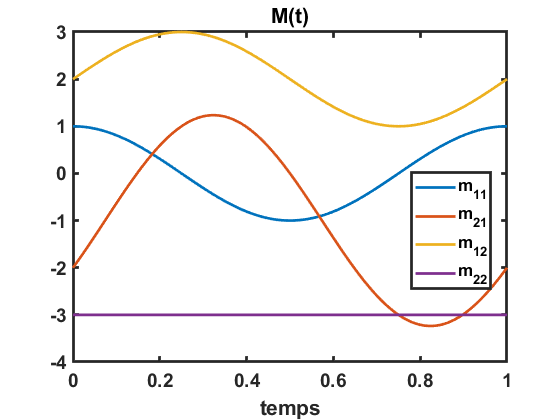
\includegraphics[width=0.45\textwidth]{demoMt.png}
\caption{Coeeficients de M évalués grace à matlab et au calcul tensoriel contracté}
\end{figure}

A noter la convention suivantes : quelque soit la dimention qui stocke les phaseurs d'un signal (dim 1 pour la fourier d'un scalaire, ou la base temporelle $e(t)$, dim3 pour les matrices... ), les m premiers coeeficients stockes les phaseurs négatifs. 

\subsection{Produit de deux matrices}


Si $A,B$ sont deux matrices $T$-périodiques, $AB$ est $T$ périodique. Alors le phaseurs de $AB$ s'exprime par la convolution matricielle : 

\begin{equation}
AB_{k} = \sum_{l\in Z} A_{l} B_{k-l} 
\end{equation}

On suppose désormais que l'on travaille avec des matrices tronquées à l'ordre m, et leur représentation 3D $\mathfrak{A}$ et $\mathfrak{B}$ : 

\begin{align}
\forall k \in [-m : m]\quad AB_{k} &= \sum_{l\in [-m: m]} A_{l} B_{k-l} \\
									&= \sum_{\scalemath{0.6}{\begin{cases}-m \leq l \leq m \\ -m \leq k-l \leq m\end{cases}}} \mathfrak{A}(:,:,m+1+l) \mathfrak{B}(:,:,m+1+k-l)\\
									&= \sum_{\scalemath{0.6}{\begin{cases}-m \leq l \leq m \\ -m \leq k-l \leq m\end{cases}}} \mathrm{flip}\left(\mathfrak{A}\right)(:,:,m+1-l) \mathfrak{B}(:,:,m+1-l+k)\\
									&= \sum_{\scalemath{0.6}{\begin{cases}1 \leq \sigma \leq 2m+1 \\ 1 \leq k+\sigma \leq 2m+1\end{cases}}} \mathrm{flip}\left(\mathfrak{A}\right)(:,:,\sigma) \mathfrak{B}(:,:,\sigma+k)\\
									&= \sum_{\scalemath{0.6}{\max (1,1-k) \leq \sigma \leq \min (2m+1,2m+1-k) }} \mathrm{flip}\left(\mathfrak{A}\right)(:,:,\sigma) \mathfrak{B}(:,:,\sigma+k)
\end{align}

Via matlab et tensorprod on peut aisément définir ce produit, le code suivant produit le produit de 2 3D array de phaseurs de dimensions compatibles, tronqué à des ordres différents, en considérant que tout phaseur au dela de la troncature est nul. 

% This file was automatically created from the m-file 
% "m2tex.m" written by USL. 
% The fontencoding in this file is UTF-8. 
%  
% You will need to include the following two packages in 
% your LaTeX-Main-File. 
%  
% \usepackage{color} 
% \usepackage{fancyvrb} 
%  
% It is advised to use the following option for Inputenc 
% \usepackage[utf8]{inputenc} 
%  
  
% definition of matlab colors: 
\definecolor{mblue}{rgb}{0,0,1} 
\definecolor{mgreen}{rgb}{0.13333,0.5451,0.13333} 
\definecolor{mred}{rgb}{0.62745,0.12549,0.94118} 
\definecolor{mgrey}{rgb}{0.5,0.5,0.5} 
\definecolor{mdarkgrey}{rgb}{0.25,0.25,0.25} 
  
\DefineShortVerb[fontfamily=courier,fontseries=m]{\$} 
\DefineShortVerb[fontfamily=courier,fontseries=b]{\#} 
  
\noindent                       
 \hspace*{-1.6em}{\scriptsize 1}$  $\color{mblue}$function$\color{black}$ D = hmq_times(A,B)$\\
 \hspace*{-1.6em}{\scriptsize 2}$  $\color{mgreen}$%Takes 2 3D array as input, seen as a Matrix sequence indexed on Z and$\color{black}$$\\
 \hspace*{-1.6em}{\scriptsize 3}$  $\color{mgreen}$%truncated, stored along the third dimension. $\color{black}$$\\
 \hspace*{-1.6em}{\scriptsize 4}$  $\color{mgreen}$%Compute the matrix convolution$\color{black}$$\\
 \hspace*{-1.6em}{\scriptsize 5}$  $\color{mgreen}$%$\color{black}$$\\
 \hspace*{-1.6em}{\scriptsize 6}$  $\color{mgreen}$% A is a 3D array of size m x n x mA$\color{black}$$\\
 \hspace*{-1.6em}{\scriptsize 7}$  $\color{mgreen}$% B is a 3D array of size n x p x mB$\color{black}$$\\
 \hspace*{-1.6em}{\scriptsize 8}$  $\color{mgreen}$%$\color{black}$$\\
 \hspace*{-1.6em}{\scriptsize 9}$      mA=(size(A,3)-1)/2;$\\
 \hspace*{-2em}{\scriptsize 10}$      mB=(size(B,3)-1)/2;$\\
 \hspace*{-2em}{\scriptsize 11}$      m=max(mB,mA);$\\
 \hspace*{-2em}{\scriptsize 12}$      D=zeros(size(A,1),size(B,2),2*m+1);$\\
 \hspace*{-2em}{\scriptsize 13}$      $\\
 \hspace*{-2em}{\scriptsize 14}$      $\color{mgreen}$%Convolution using tensorprod$\color{black}$$\\
 \hspace*{-2em}{\scriptsize 15}$      $\color{mblue}$for$\color{black}$ k=(-m:m)$\\
 \hspace*{-2em}{\scriptsize 16}$          l1=max(k-mB,-mA);$\\
 \hspace*{-2em}{\scriptsize 17}$          l2=min(k+mB,mA);$\\
 \hspace*{-2em}{\scriptsize 18}$          V=A(:,:,(mA+1+l1):(mA+1+l2));$\\
 \hspace*{-2em}{\scriptsize 19}$          U=B(:,:,(k+mB+1-l1):-1:(k+mB+1-l2));$\\
 \hspace*{-2em}{\scriptsize 20}$          D(:,:,m+1+k)=tensorprod(V,U,[2,3],[1,3]);$\\
 \hspace*{-2em}{\scriptsize 21}$      $\color{mblue}$end$\color{black}$$\\
 \hspace*{-2em}{\scriptsize 22}$  $\\
 \hspace*{-2em}{\scriptsize 23}$  $\color{mblue}$end$\color{black}$$\\ 
  
\UndefineShortVerb{\$} 
\UndefineShortVerb{\#}


\subsection{Représentation des matrices Toeplitz}

On différencie 2 types de matrices associés aux phaseurs de $M(t)$ : 
\begin{itemize}
\item la matrice \emph{Toeplitz par blocs} (anglais : block Toeplitz matrix), où des blocs sont répétés sur les diagonales
\item la matrice en \emph{Blocs-Toeplitzs} (anglais Toeplitz blocks matrix), qui est une matrice par bloc dont chacun des blocs est une matrice Toeplitz
\end{itemize}

\begin{figure}[h!]
\begin{equation}
    A = 
\begin{pmatrix}
a_{11} & a_{12} & \cdots & a_{1n}\\
a_{21} & \ddots & & \vdots\\
\vdots \\
a_{m1} & & & a_{mn}
\end{pmatrix} 
\end{equation}
\caption*{Matrice A dont les coefficients dépendent du temps }
\end{figure}


\begin{figure}[h!]
\begin{equation}
\cToep{A}  = 
\left[\begin{array}{c|c|c|c}
\Toep{a_{11}} & \Toep{a_{12}} & \cdots  & \Toep{a_{1n}}\\ \hline
\Toep{a_{21}} & \ddots  & & \\ \hline
\vdots &  & & \\ \hline
\Toep{a_{m1}} & & &  \Toep{a_{mn}}   \\
\end{array} \right] 
\end{equation} 
\caption*{Représentation en blocs Toeplitzs }
\end{figure}


\begin{figure}[h!]
\begin{align}
    \mToep{A} = \begin{pmatrix}
    \ddots & \ddots &  \ddots &  \\
        \ddots&A_0 & A_{-1} & A_{-2} \\
        \ddots &A_1 & A_{0} & A_{-1}&\ddots \\
        &A_2 & A_{1} & A_{0} &\ddots\\
        &&\ddots &\ddots &\ddots\\       
        & &  &  
    \end{pmatrix}
    \end{align}
\caption*{Représentation Toeplitz par bloc }
\end{figure}
\end{document}
